\section{Constant Coefficient Homogeneous Systems II}

\noindent
We saw in Section~10.4 that if an $n\times n$ constant matrix $A$ has $n$ real eigenvalues
$\lambda_{1}$, $\lambda_{2}$, \dots, $\lambda_{n}$ (which need not be distinct) with associated
linearly independent eigenvectors ${\bf x}_{1}$, ${\bf x}_{2}$, \dots, ${\bf x}_{n}$, then the
general solution of ${\bf y}'=A{\bf y}$ is
\[
  {\bf y}=c_{1}{\bf x}_{1}e^{\lambda_{1}t}+c_{2}{\bf x}_{2}e^{\lambda_{2}t}+\cdots+c_{n}{\bf x}_{n}e^{\lambda_{n}t}.
\]
In this section we consider the case where $A$ has $n$ real eigenvalues, but does not have $n$
linearly independent eigenvectors. It is shown in linear algebra that this occurs if and only if $A$
has at least one eigenvalue of multiplicity $r>1$ such that the associated eigenspace has dimension
less than $r$. In this case $A$ is said to be {\color{blue}\it defective\/}. Since it's beyond the
scope of this book to give a complete analysis of systems with defective coefficient matrices, we
will restrict our attention to some commonly occurring special cases.

\begin{example}
  \label{example:10.5.1}\rm \space Show that the system
  \begin{equation}
    \label{eq:10.5.1}{\bf y}'=\twobytwo{11}{-25}4{-9}{\bf y}
  \end{equation}
  does not have a fundamental set of solutions of the form
  $\{{\bf x}_{1}e^{\lambda_{1}t},{\bf x}_{2}e^{\lambda_{2}t}\}$, where $\lambda_{1}$ and
  $\lambda_{2}$ are eigenvalues of the coefficient matrix $A$ of \eqref{eq:10.5.1} and
  ${\bf x}_{1}$ and ${\bf x}_{2}$ are associated linearly independent eigenvectors.
\end{example}

\solution The characteristic polynomial of $A$ is
\begin{eqnarray*}
  \twochar{11}{-25}4{-9} & = & (\lambda-11)(\lambda+9)+100 \\
                         & = & \lambda^{2}-2\lambda+1=(\lambda-1)^{2}.
\end{eqnarray*}
Hence, $\lambda=1$ is the only eigenvalue of $A$. The augmented matrix of the system
$(A-I){\bf x}={\bf0}$ is
\[
  \left[
  \begin{array}{rrcr}
    10 & -25 & \vdots & 0 \\
    4  & -10 & \vdots & 0
  \end{array}\right],
\]
which is row equivalent to
\[
  \left[
  \begin{array}{rrcr}
    1 & -\dst\frac{5}{2} & \vdots & 0 \\[10pt]
    0 & 0                & \vdots & 0
  \end{array}\right].
\]
Hence, $x_{1}=5x_{2}/2$ where $x_{2}$ is arbitrary. Therefore all eigenvectors of $A$ are scalar
multiples of ${\bf x}_{1}=\dst{\twocol52}$, so $A$ does not have a set of two linearly independent
eigenvectors. \bbox

From Example~\ref{example:10.5.1}, we know that all scalar multiples of
${\bf y}_{1}=\dst{\twocol52}e^{t}$ are solutions of \eqref{eq:10.5.1}; however, to find the general
solution we must find a second solution ${\bf y}_{2}$ such that $\{{\bf y}_{1},{\bf y}_{2}\}$ is
linearly independent. Based on your recollection of the procedure for solving a constant coefficient
scalar equation
\[
  ay''+by'+cy=0
\]
in the case where the characteristic polynomial has a repeated root, you might expect to obtain a
second solution of \eqref{eq:10.5.1} by multiplying the first solution by $t$. However, this yields
${\bf y}_{2}=\dst{\twocol52}te^{t}$, which doesn't work, since
\[
  {\bf y}_{2}'=\twocol52(te^{t}+e^{t}),\mbox{\quad while \quad }\twobytwo{11}{-25}4{-9}{\bf y}_{2}=\twocol52te^{t}.
\]

The next theorem shows what to do in this situation.

\begin{theorem}
  \color{blue}
  \label{thmtype:10.5.1} Suppose the $n\times n$ matrix $A$ has an eigenvalue $\lambda_{1}$ of
  multiplicity $\ge2$ and the associated eigenspace has dimension $1$; that is, all
  $\lambda_{1}$-eigenvectors of $A$ are scalar multiples of an eigenvector ${\bf x}$. Then there are
  infinitely many vectors ${\bf u}$ such that
  \begin{equation}
    \label{eq:10.5.2}(A-\lambda_{1}I){\bf u}={\bf x}.
  \end{equation}
  Moreover, if ${\bf u}$ is any such vector then
  \begin{equation}
    \label{eq:10.5.3}{\bf y}_{1}={\bf x}e^{\lambda_{1}t}\quad\mbox{and }\quad{\bf y}_{2}={\bf u}e^{\lambda_{1}t}+{\bf x}te^{\lambda_{1}t}
  \end{equation}
  are linearly independent solutions of ${\bf y}'=A{\bf y}$.
\end{theorem}

A complete proof of this theorem is beyond the scope of this book. The difficulty is in proving that
there's a vector ${\bf u}$ satisfying \eqref{eq:10.5.2}, since $\det(A-\lambda_{1}I)=0$. We'll take
this without proof and verify the other assertions of the theorem.

We already know that ${\bf y}_{1}$ in \eqref{eq:10.5.3} is a solution of ${\bf y}'=A{\bf y}$. To see
that ${\bf y}_{2}$ is also a solution, we compute
\begin{eqnarray*}
  {\bf y}_{2}'-A{\bf y}_{2} & = & \lambda_{1}{\bf u}e^{\lambda_{1}t}+{\bf x}e^{\lambda_{1}t}+\lambda_{1}{\bf x}te^{\lambda_{1}t}-A{\bf u}e^{\lambda_{1}t}-A{\bf x}te^{\lambda_{1}t} \\
                            & = & (\lambda_{1}{\bf u}+{\bf x}-A{\bf u})e^{\lambda_{1}t}+(\lambda_{1}{\bf x}-A{\bf x})te^{\lambda_{1}t}.
\end{eqnarray*}
Since $A{\bf x}=\lambda_{1}{\bf x}$, this can be written as
\[
  {\bf y}_{2}'-A{\bf y}_{2}=- \left((A-\lambda_{1}I){\bf u}-{\bf x}\right)e^{\lambda_{1}t},
\]
and now \eqref{eq:10.5.2} implies that ${\bf y}_{2}'=A{\bf y}_{2}$.

To see that ${\bf y}_{1}$ and ${\bf y}_{2}$ are linearly independent, suppose $c_{1}$ and $c_{2}$
are constants such that
\begin{equation}
  \label{eq:10.5.4}c_{1}{\bf y}_{1}+c_{2}{\bf y}_{2}=c_{1}{\bf x}e^{\lambda_{1}t}+c_{2}({\bf u}e^{\lambda_{1}t}+{\bf x}te^{\lambda_{1}t})={\bf0}.
\end{equation}
We must show that $c_{1}=c_{2}=0$. Multiplying \eqref{eq:10.5.4} by $e^{-\lambda_{1}t}$ shows that
\begin{equation}
  \label{eq:10.5.5}c_{1}{\bf x}+c_{2}({\bf u}+{\bf x}t)={\bf0}.
\end{equation}
By differentiating this with respect to $t$, we see that $c_{2}{\bf x}={\bf0}$, which implies
$c_{2}=0$, because ${\bf x}\ne{\bf0}$. Substituting $c_{2}=0$ into \eqref{eq:10.5.5} yields
$c_{1}{\bf x}={\bf0}$, which implies that $c_{1}=0$, again because ${\bf x}\ne{\bf0}$.
\begin{example}
  \label{example:10.5.2}\rm Use Theorem~\ref{thmtype:10.5.1} to find the general solution of the
  system
  \begin{equation}
    \label{eq:10.5.6}{\bf y}'=\twobytwo{11}{-25}4{-9}{\bf y}
  \end{equation}
  considered in Example~\ref{example:10.5.1}.
\end{example}

\solution In Example~\ref{example:10.5.1} we saw that $\lambda_{1}=1$ is an eigenvalue of
multiplicity $2$ of the coefficient matrix $A$ in \eqref{eq:10.5.6}, and that all of the
eigenvectors of $A$ are multiples of
\[
  {\bf x}=\twocol52.
\]
Therefore
\[
  {\bf y}_{1}=\twocol52e^{t}
\]
is a solution of \eqref{eq:10.5.6}. From Theorem~\ref{thmtype:10.5.1}, a second solution is given by
${\bf y}_{2}={\bf u}e^{t}+{\bf x}te^{t}$, where $(A-I){\bf u}={\bf x}$. The augmented matrix of this
system is
\[
  \left[
  \begin{array}{rrcr}
    10 & -25 & \vdots & 5 \\
    4  & -10 & \vdots & 2
  \end{array}\right],
\]
which is row equivalent to
\[
  \dst{\left[\begin{array}{rrcr}1&-\frac{5}{2}&\vdots&1\over2\\ 0&0&\vdots&0\end{array}\right]}.
\]
Therefore the components of ${\bf u}$ must satisfy
\[
  u_{1}-\frac{5}{2}u_{2}=\frac{1}{2},
\]
where $u_{2}$ is arbitrary. We choose $u_{2}=0$, so that $u_{1}=1/2$ and
\[
  {\bf u}=\twocol{\frac{1}{2}}0.
\]
Thus,
\[
  {\bf y}_{2}=\twocol10{\frac{e^{t}}{2}}+\twocol52te^{t}.
\]
Since ${\bf y}_{1}$ and ${\bf y}_{2}$ are linearly independent by Theorem~\ref{thmtype:10.5.1}, they
form a fundamental set of solutions of \eqref{eq:10.5.6}. Therefore the general solution of
\eqref{eq:10.5.6} is
\[
  {\bf y}=c_{1}\twocol52e^{t}+c_{2}\left(\twocol10{\frac{e^{t}}{2}}+\twocol52te^{t}\right).\bbox
\]

Note that choosing the arbitrary constant $u_{2}$ to be nonzero is equivalent to adding a scalar
multiple of ${\bf y}_{1}$ to the second solution ${\bf y}_{2}$ (Exercise~\ref{exer:10.5.33}).

\begin{example}
  \label{example:10.5.3}\rm Find the general solution of
  \begin{equation}
    \label{eq:10.5.7}{\bf y}'=\threebythree34{-10}21{-2}22{-5}{\bf y}.
  \end{equation}
\end{example}

\solution The characteristic polynomial of the coefficient matrix $A$ in \eqref{eq:10.5.7} is
\[
  \left|
  \begin{array}{ccc}
    3-\lambda & 4         & -10        \\
    2         & 1-\lambda & -2         \\
    2         & 2         & -5-\lambda
  \end{array}\right|=- (\lambda-1)(\lambda+1)^{2}.
\]
Hence, the eigenvalues are $\lambda_{1}=1$ with multiplicity~$1$ and $\lambda_{2}=-1$ with
multiplicity~$2$.

Eigenvectors associated with $\lambda_{1}=1$ must satisfy $(A-I){\bf x}={\bf0}$. The augmented
matrix of this system is
\[
  \left[
  \begin{array}{rrrcr}
    2 & 4 & -10 & \vdots & 0 \\
    2 & 0 & -2  & \vdots & 0 \\
    2 & 2 & -6  & \vdots & 0
  \end{array}\right],
\]
which is row equivalent to
\[
  \left[
  \begin{array}{rrrcr}
    1 & 0 & -1 & \vdots & 0 \\
    0 & 1 & -2 & \vdots & 0 \\
    0 & 0 & 0  & \vdots & 0
  \end{array}\right].
\]
Hence, $x_{1}=x_{3}$ and $x_{2}=2x_{3}$, where $x_{3}$ is arbitrary. Choosing $x_{3}=1$ yields the
eigenvector
\[
  {\bf x}_{1}=\threecol121.
\]
Therefore
\[
  {\bf y}_{1}=\threecol121e^{t}
\]
is a solution of \eqref{eq:10.5.7}.

Eigenvectors associated with $\lambda_{2}=-1$ satisfy $(A+I){\bf x}={\bf0}$. The augmented matrix of
this system is
\[
  \left[
  \begin{array}{rrrcr}
    4 & 4 & -10 & \vdots & 0 \\
    2 & 2 & -2  & \vdots & 0 \\
    2 & 2 & -4  & \vdots & 0
  \end{array}\right],
\]
which is row equivalent to
\[
  \left[
  \begin{array}{rrrcr}
    1 & 1 & 0 & \vdots & 0 \\
    0 & 0 & 1 & \vdots & 0 \\
    0 & 0 & 0 & \vdots & 0
  \end{array}\right].
\]
Hence, $x_{3}=0$ and $x_{1}=-x_{2}$, where $x_{2}$ is arbitrary. Choosing $x_{2}=1$ yields the
eigenvector
\[
  {\bf x}_{2}=\threecol{-1}10,
\]
so
\[
  {\bf y}_{2}=\threecol{-1}10e^{-t}
\]
is a solution of \eqref{eq:10.5.7}.

Since all the eigenvectors of $A$ associated with $\lambda_{2}=-1$ are multiples of ${\bf x}_{2}$,
we must now use Theorem~\ref{thmtype:10.5.1} to find a third solution of \eqref{eq:10.5.7} in the
form
\begin{equation}
  \label{eq:10.5.8}{\bf y}_{3}={\bf u}e^{-t}+\threecol{-1}10te^{-t},
\end{equation}
where ${\bf u}$ is a solution of $(A+I){\bf u}={\bf x}_{2}$. The augmented matrix of this system is
\[
  \left[
  \begin{array}{rrrcr}
    4 & 4 & -10 & \vdots & -1 \\
    2 & 2 & -2  & \vdots & 1  \\
    2 & 2 & -4  & \vdots & 0
  \end{array}\right],
\]
which is row equivalent to
\[
  \left[
  \begin{array}{rrrcr}
    1 & 1 & 0 & \vdots & 1           \\
    0 & 0 & 1 & \vdots & \frac{1}{2} \\
    0 & 0 & 0 & \vdots & 0
  \end{array}\right].
\]
Hence, $u_{3}=1/2$ and $u_{1}=1-u_{2}$, where $u_{2}$ is arbitrary. Choosing $u_{2}=0$ yields
\[
  {\bf u}=\threecol10{\frac{1}{2}},
\]
and substituting this into \eqref{eq:10.5.8} yields the solution
\[
  {\bf y}_{3}=\threecol201{\frac{e^{-t}}{2}}+\threecol{-1}10te^{-t}
\]
of \eqref{eq:10.5.7}.

Since the Wronskian of $\{{\bf y}_{1},{\bf y}_{2},{\bf y}_{3}\}$ at $t=0$ is
\[
  \left|
  \begin{array}{rrr}
    1 & -1 & 1       \\
    2 & 1  & 0       \\
    1 & 0  & 1\over2
  \end{array}\right|=\frac{1}{2},
\]
$\{{\bf y}_{1},{\bf y}_{2},{\bf y}_{3}\}$ is a fundamental set of solutions of \eqref{eq:10.5.7}.
Therefore the general solution of \eqref{eq:10.5.7} is
\[
  {\bf y}=c_{1}\threecol121e^{t}+c_{2}\threecol{-1}10e^{-t}+c_{3}\left (\threecol201{\frac{e^{-t}}{2}}+\threecol{-1}10te^{-t}\right).
\]

\begin{theorem}
  \color{blue}
  \label{thmtype:10.5.2} Suppose the $n\times n$ matrix $A$ has an eigenvalue $\lambda_{1}$ of
  multiplicity $\ge3$ and the associated eigenspace is one--dimensional; that is, all eigenvectors
  associated with $\lambda_{1}$ are scalar multiples of the eigenvector ${\bf x}$. Then there are
  infinitely many vectors ${\bf u}$ such that
  \begin{equation}
    \label{eq:10.5.9}(A-\lambda_{1}I){\bf u}={\bf x},
  \end{equation}
  and, if ${\bf u}$ is any such vector, there are infinitely many vectors ${\bf v}$ such that
  \begin{equation}
    \label{eq:10.5.10}(A-\lambda_{1}I){\bf v}={\bf u}.
  \end{equation}
  If ${\bf u}$ satisfies {\rm\eqref{eq:10.5.9}} and ${\bf v}$ satisfies {\rm\eqref{eq:10.5.10}},
  then
  \begin{eqnarray*}
    {\bf y}_{1} & = & {\bf x}e^{\lambda_{1}t},                                      \\
    {\bf y}_{2} & = & {\bf u}e^{\lambda_{1}t}+{\bf x}te^{\lambda_{1}t},\mbox{ and } \\
    {\bf y}_{3} & = & {\bf v}e^{\lambda_{1}t}+{\bf u}te^{\lambda_{1}t}+{\bf x}{\frac{t^{2}e^{\lambda_{1}t}}{2}}
  \end{eqnarray*}
  are linearly independent solutions of ${\bf y}'=A{\bf y}$.
\end{theorem}

Again, it's beyond the scope of this book to prove that there are vectors ${\bf u}$ and ${\bf v}$
that satisfy \eqref{eq:10.5.9} and \eqref{eq:10.5.10}. Theorem~\ref{thmtype:10.5.1} implies that
${\bf y}_{1}$ and ${\bf y}_{2}$ are solutions of ${\bf y}'=A{\bf y}$. We leave the rest of the proof
to you (Exercise~\ref{exer:10.5.34}).

\begin{example}
  \label{example:10.5.4}\rm Use Theorem~\ref{thmtype:10.5.2} to find the general solution of
  \begin{equation}
    \label{eq:10.5.11}{\bf y}'=\threebythree11113{-1}022{\bf y}.
  \end{equation}
\end{example}

\solution The characteristic polynomial of the coefficient matrix $A$ in \eqref{eq:10.5.11} is
\[
  \left|
  \begin{array}{ccc}
    1-\lambda & 1         & \phantom{-}1 \\
    1         & 3-\lambda & -1           \\
    0         & 2         & 2-\lambda
  \end{array}\right|=-(\lambda-2)^{3}.
\]
Hence, $\lambda_{1}=2$ is an eigenvalue of multiplicity $3$. The associated eigenvectors satisfy
$(A-2I){\bf x}={\bf0}$. The augmented matrix of this system is
\[
  \left[
  \begin{array}{rrrcr}
    -1 & 1 & 1  & \vdots & 0 \\
    1  & 1 & -1 & \vdots & 0 \\
    0  & 2 & 0  & \vdots & 0
  \end{array}\right],
\]
which is row equivalent to
\[
  \left[
  \begin{array}{rrrcr}
    1 & 0 & -1 & \vdots & 0 \\
    0 & 1 & 0  & \vdots & 0 \\
    0 & 0 & 0  & \vdots & 0
  \end{array}\right].
\]
Hence, $x_{1}=x_{3}$ and $x_{2}=0$, so the eigenvectors are all scalar multiples of
\[
  {\bf x}_{1}=\threecol101.
\]
Therefore
\[
  {\bf y}_{1}=\threecol101e^{2t}
\]
is a solution of \eqref{eq:10.5.11}.

We now find a second solution of \eqref{eq:10.5.11} in the form
\[
  {\bf y}_{2}={\bf u}e^{2t}+\threecol101te^{2t},
\]
where ${\bf u}$ satisfies $(A-2I){\bf u}={\bf x}_{1}$. The augmented matrix of this system is
\[
  \left[
  \begin{array}{rrrcr}
    -1 & 1 & 1  & \vdots & 1 \\
    1  & 1 & -1 & \vdots & 0 \\
    0  & 2 & 0  & \vdots & 1
  \end{array}\right],
\]
which is row equivalent to
\[
  \left[
  \begin{array}{rrrcr}
    1 & 0 & -1 & \vdots & -\frac{1}{2} \\
    0 & 1 & 0  & \vdots & \frac{1}{2}  \\
    0 & 0 & 0  & \vdots & 0
  \end{array}\right].
\]
Letting $u_{3}=0$ yields $u_{1}=-1/2$ and $u_{2}=1/2$; hence,
\[
  {\bf u}=\frac{1}{2}\threecol{-1}10
\]
and
\[
  {\bf y}_{2}=\threecol{-1}10{\frac{e^{2t}}{2}}+\threecol101te^{2t}
\]
is a solution of \eqref{eq:10.5.11}.

We now find a third solution of \eqref{eq:10.5.11} in the form
\[
  {\bf y}_{3}={\bf v}e^{2t}+\threecol{-1}10{\frac{te^{2t}}{2}}+\threecol101{\frac{t^{2}e^{2t}}{2}}
\]
where ${\bf v}$ satisfies $(A-2I){\bf v}={\bf u}$. The augmented matrix of this system is
\[
  \left[
  \begin{array}{rrrcr}
    -1 & 1 & 1  & \vdots & -\frac{1}{2} \\
    1  & 1 & -1 & \vdots & \frac{1}{2}  \\
    0  & 2 & 0  & \vdots & 0
  \end{array}\right],
\]
which is row equivalent to
\[
  \left[
  \begin{array}{rrrcr}
    1 & 0 & -1 & \vdots & \frac{1}{2} \\
    0 & 1 & 0  & \vdots & 0           \\
    0 & 0 & 0  & \vdots & 0
  \end{array}\right].
\]
Letting $v_{3}=0$ yields $v_{1}=1/2$ and $v_{2}=0$; hence,
\[
  {\bf v}=\frac{1}{2}\threecol100.
\]
Therefore
\[
  {\bf y}_{3}=\threecol100{\frac{e^{2t}}{2}}+ \threecol{-1}10{\frac{te^{2t}}{2}}+\threecol101{\frac{t^{2}e^{2t}}{2}}
\]
is a solution of \eqref{eq:10.5.11}. Since ${\bf y}_{1}$, ${\bf y}_{2}$, and ${\bf y}_{3}$ are
linearly independent by Theorem~\ref{thmtype:10.5.2}, they form a fundamental set of solutions of
\eqref{eq:10.5.11}. Therefore the general solution of \eqref{eq:10.5.11} is
\begin{eqnarray*}
  {\bf y} & = & \dst{c_{1}\threecol101e^{2t}+c_{2}\left(\threecol{-1}10{\frac{e^{2t}}{2}}+\threecol101te^{2t}\right)} \\[2\jot]
          &   & +c_{3}\dst{\left(\threecol100{\frac{e^{2t}}{2}}+\threecol{-1}10{\frac{te^{2t}}{2}}+\threecol101{\frac{t^{2}e^{2t}}{2}}\right)}.
\end{eqnarray*}

\enlargethispage{1in}

\begin{theorem}
  \color{blue}
  \label{thmtype:10.5.3} Suppose the $n\times n$ matrix $A$ has an eigenvalue $\lambda_{1}$ of
  multiplicity $\ge3$ and the associated eigenspace is two--dimensional; that is, all eigenvectors
  of $A$ associated with $\lambda_{1}$ are linear combinations of two linearly independent
  eigenvectors ${\bf x}_{1}$ and ${\bf x}_{2}$. Then there are constants $\alpha$ and $\beta$ (not
  both zero) such that if
  \begin{equation}
    \label{eq:10.5.12}{\bf x}_{3}=\alpha{\bf x}_{1}+\beta{\bf x}_{2},
  \end{equation}
  then there are infinitely many vectors ${\bf u}$ such that
  \begin{equation}
    \label{eq:10.5.13}(A-\lambda_{1}I){\bf u}={\bf x}_{3}.
  \end{equation}
  If ${\bf u}$ satisfies {\rm\eqref{eq:10.5.13}}, then
  \begin{eqnarray}
    {\bf y}_{1} & = & {\bf x}_{1}e^{\lambda_{1}t},\nonumber            \\
    {\bf y}_{2} & = & {\bf x}_{2}e^{\lambda_{1}t},\mbox{and }\nonumber \\
    {\bf y}_{3} & = & {\bf u}e^{\lambda_{1}t}+{\bf x}_{3}te^{\lambda_{1}t}\label{eq:10.5.14},
  \end{eqnarray}
  are linearly independent solutions of ${\bf y}'=A{\bf y}$.
\end{theorem}

We omit the proof of this theorem.

\newpage

\begin{example}
  \label{example:10.5.5}\rm Use Theorem~\ref{thmtype:10.5.3} to find the general solution of
  \begin{equation}
    \label{eq:10.5.15}{\bf y}'=\threebythree001{-1}11{-1}02{\bf y}.
  \end{equation}
\end{example}

\solution The characteristic polynomial of the coefficient matrix $A$ in \eqref{eq:10.5.15} is
\[
  \left|
  \begin{array}{ccc}
    -\lambda & 0         & 1         \\
    -1       & 1-\lambda & 1         \\
    -1       & 0         & 2-\lambda
  \end{array}\right|=-(\lambda-1)^{3}.
\]
Hence, $\lambda_{1}=1$ is an eigenvalue of multiplicity $3$. The associated eigenvectors satisfy
$(A-I){\bf x}={\bf 0}$. The augmented matrix of this system is
\[
  \left[
  \begin{array}{rrrcr}
    -1 & 0 & 1 & \vdots & 0 \\
    -1 & 0 & 1 & \vdots & 0 \\
    -1 & 0 & 1 & \vdots & 0
  \end{array}\right],
\]
which is row equivalent to
\[
  \left[
  \begin{array}{rrrcr}
    1 & 0 & -1 & \vdots & 0 \\
    0 & 0 & 0  & \vdots & 0 \\
    0 & 0 & 0  & \vdots & 0
  \end{array}\right].
\]
Hence, $x_{1}=x_{3}$ and $x_{2}$ is arbitrary, so the eigenvectors are of the form
\[
  {\bf x}=\threecol{x_{3}}{x_{2}}{x_{3}}=x_{3}\threecol101+x_{2}\threecol010.
\]
Therefore the vectors
\begin{equation}
  \label{eq:10.5.16}{\bf x}_{1}=\threecol101\quad\mbox{and }\quad{\bf x}_{2}=\threecol010
\end{equation}
form a basis for the eigenspace, and
\[
  {\bf y}_{1}=\threecol101e^{t}\quad\mbox{and }\quad{\bf y}_{2}=\threecol010e^{t}
\]
are linearly independent solutions of \eqref{eq:10.5.15}.

To find a third linearly independent solution of \eqref{eq:10.5.15}, we must find constants $\alpha$
and $\beta$ (not both zero) such that the system
\begin{equation}
  \label{eq:10.5.17}(A-I){\bf u}=\alpha{\bf x}_{1}+\beta{\bf x}_{2}
\end{equation}
has a solution ${\bf u}$. The augmented matrix of this system is
\[
  \left[
  \begin{array}{rrrcr}
    -1 & 0 & 1 & \vdots & \alpha \\
    -1 & 0 & 1 & \vdots & \beta  \\
    -1 & 0 & 1 & \vdots & \alpha
  \end{array}\right],
\]
which is row equivalent to
\begin{equation}
  \label{eq:10.5.18}\left[
  \begin{array}{rrrcr}
    1 & 0 & -1 & \vdots & -\alpha      \\
    0 & 0 & 0  & \vdots & \beta-\alpha \\
    0 & 0 & 0  & \vdots & 0
  \end{array}
  \right].
\end{equation}
Therefore \eqref{eq:10.5.17} has a solution if and only if $\beta=\alpha$, where $\alpha$ is
arbitrary. If $\alpha=\beta=1$ then \eqref{eq:10.5.12} and \eqref{eq:10.5.16} yield
\[
  {\bf x}_{3}={\bf x}_{1}+{\bf x}_{2}= \threecol101+\threecol010=\threecol111,
\]
and the augmented matrix \eqref{eq:10.5.18} becomes
\[
  \left[
  \begin{array}{rrrcr}
    1 & 0 & -1 & \vdots & -1 \\
    0 & 0 & 0  & \vdots & 0  \\
    0 & 0 & 0  & \vdots & 0
  \end{array}
  \right].
\]
This implies that $u_{1}=-1+u_{3}$, while $u_{2}$ and $u_{3}$ are arbitrary. Choosing
$u_{2}=u_{3}=0$ yields
\[
  {\bf u}=\threecol{-1}00.
\]
Therefore \eqref{eq:10.5.14} implies that
\[
  {\bf y}_{3}={\bf u}e^{t}+{\bf x}_{3}te^{t}=\threecol{-1}00e^{t}+\threecol111te^{t}
\]
is a solution of \eqref{eq:10.5.15}. Since ${\bf y}_{1}$, ${\bf y}_{2}$, and ${\bf y}_{3}$ are
linearly independent by Theorem~\ref{thmtype:10.5.3}, they form a fundamental set of solutions for
\eqref{eq:10.5.15}. Therefore the general solution of \eqref{eq:10.5.15} is
\[
  {\bf y}=c_{1}\threecol101e^{t}+c_{2}\threecol010e^{t}+c_{3}\left(\threecol{-1}00e^{t}+\threecol111te^{t}\right).\bbox
\]

\boxit{Geometric Properties of Solutions when $n=2$}

\noindent
We'll now consider the geometric properties of solutions of a $2\times2$ constant coefficient system
\begin{equation}
  \label{eq:10.5.19}\twocol{y_{1}'}{y_{2}'}=\left[
  \begin{array}{cc}
    a_{11} & a_{12} \\
    a_{21} & a_{22}
  \end{array}\right]\twocol{y_{1}}{y_{2}}
\end{equation}
under the assumptions of this section; that is, when the matrix
\[
  A=\left[
  \begin{array}{cc}
    a_{11} & a_{12} \\
    a_{21} & a_{22}
  \end{array}\right]
\]
has a repeated eigenvalue $\lambda_{1}$ and the associated eigenspace is one-dimensional. In this
case we know from Theorem~\ref{thmtype:10.5.1} that the general solution of \eqref{eq:10.5.19} is
\begin{equation}
  \label{eq:10.5.20}{\bf y}=c_{1}{\bf x}e^{\lambda_{1}t}+c_{2}({\bf u}e^{\lambda_{1}t}+{\bf x}te^{\lambda_{1}t}),
\end{equation}
where ${\bf x}$ is an eigenvector of $A$ and ${\bf u}$ is any one of the infinitely many solutions
of
\begin{equation}
  \label{eq:10.5.21}(A-\lambda_{1}I){\bf u}={\bf x}.
\end{equation}
We assume that $\lambda_{1}\ne0$.

\begin{figure}[H]
  \centering
  \scalebox{.8}{
  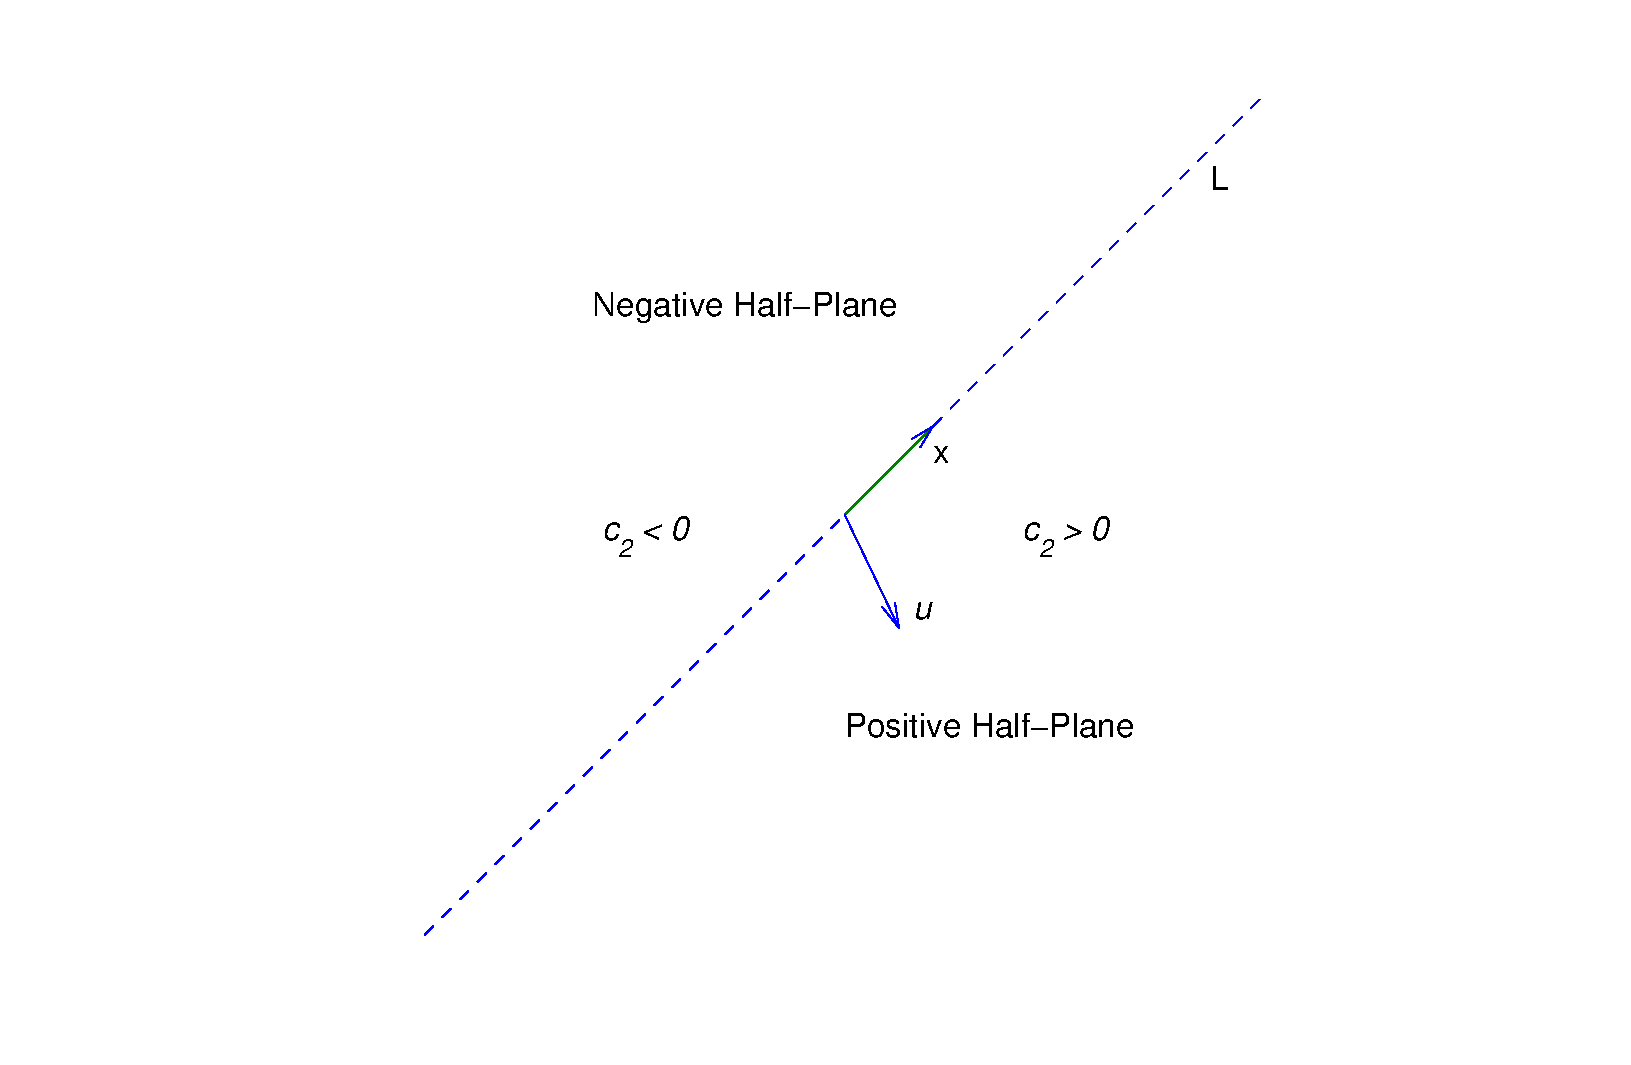
\includegraphics[bb=-78 148 689 643, width=5.67in, height=3.66in, keepaspectratio]{fig100501}}
  \caption{Positive and negative half-planes}
  \label{figure:10.5.1}
\end{figure}

Let $L$ denote the line through the origin parallel to ${\bf x}$. By a {\color{blue}\it half-line\/}
of $L$ we mean either of the rays obtained by removing the origin from $L$. Eqn.~\eqref{eq:10.5.20}
is a parametric equation of the half-line of $L$ in the direction of ${\bf x}$ if $c_{1}>0$, or of
the half-line of $L$ in the direction of $-{\bf x}$ if $c_{1}<0$. The origin is the trajectory of
the trivial solution ${\bf y}\equiv{\bf0}$.

Henceforth, we assume that $c_{2}\ne0$. In this case, the trajectory of \eqref{eq:10.5.20} can't
intersect $L$, since every point of $L$ is on a trajectory obtained by setting $c_{2}=0$. Therefore
the trajectory of \eqref{eq:10.5.20} must lie entirely in one of the open half-planes bounded by
$L$, but does not contain any point on $L$. Since the initial point $(y_{1}(0),y_{2}(0))$ defined by
${\bf y}(0)=c_{1}{\bf x}+c_{2}{\bf u}$ is on the trajectory, we can determine which half-plane
contains the trajectory from the sign of $c_{2}$, as shown in Figure~\ref{figure:10.5.1}. For
convenience we'll call the half-plane where $c_{2}>0$ the {\color{blue}\it positive half-plane\/}.
Similarly, the half- plane where $c_{2}<0$ is the {\color{blue}\it negative half-plane\/}. You should
convince yourself (Exercise~\ref{exer:10.5.35}) that even though there are infinitely many vectors
${\bf u}$ that satisfy \eqref{eq:10.5.21}, they all define the same positive and negative
half-planes. In the figures simply regard ${\bf u}$ as an arrow pointing to the positive half-plane,
since we haven't attempted to give ${\bf u}$ its proper length or direction in comparison with
${\bf x}$. For our purposes here, only the relative orientation of ${\bf x}$ and ${\bf u}$ is
important; that is, whether the positive half-plane is to the right of an observer facing the
direction of ${\bf x}$ (as in Figures~\ref{figure:10.5.2} and \ref{figure:10.5.5}), or to the left
of the observer (as in Figures~\ref{figure:10.5.3} and \ref{figure:10.5.4}).

Multiplying \eqref{eq:10.5.20} by $e^{-\lambda_{1}t}$ yields
\[
  e^{-\lambda_{1}t}{\bf y}(t)=c_{1}{\bf x}+c_{2}{\bf u}+c_{2}t{\bf x}.
\]
Since the last term on the right is dominant when $|t|$ is large, this provides the following
information on the direction of ${\bf y}(t)$:
\begin{alist}
  \item % (a)
  Along trajectories in the positive half-plane ($c_{2}>0$), the direction of ${\bf y}(t)$
  approaches the direction of ${\bf x}$ as $t\to\infty$ and the direction of $-{\bf x}$ as
  $t\to-\infty$.

  \item % (b)
  Along trajectories in the negative half-plane ($c_{2}<0$), the direction of ${\bf y}(t)$
  approaches the direction of $-{\bf x}$ as $t\to\infty$ and the direction of ${\bf x}$ as
  $t\to-\infty$.
\end{alist}

Since
\[
  \lim_{t\to\infty}\|{\bf y}(t)\|=\infty\mbox{\quad and \quad}\lim_{t\to-\infty}{\bf y}(t)={\bf0}\mbox{\quad if \quad}\lambda_{1}>0,
\]
or
\[
  \lim_{t\to-\infty}\|{\bf y}(t)\|=\infty\mbox{\quad and \quad}\lim_{t\to\infty}{\bf y}(t)={\bf0}\mbox{\quad if \quad}\lambda_{1}<0,
\]
there are four possible patterns for the trajectories of \eqref{eq:10.5.19}, depending upon the
signs of $c_{2}$ and $\lambda_{1}$. Figures~\ref{figure:10.5.2}-\ref{figure:10.5.5} illustrate these
patterns, and reveal the following principle:

{\color{blue}\it If $\lambda_{1}$ and $c_{2}$ have the same sign then the direction of the trajectory
approaches the direction of $-{\bf x}$ as $\|{\bf y}\|\to0$ and the direction of ${\bf x}$ as
$\|{\bf y}\|\to\infty$. If $\lambda_{1}$ and $c_{2}$ have opposite signs then the direction of the
trajectory approaches the direction of ${\bf x}$ as $\|{\bf y}\|\to0$ and the direction of
$-{\bf x}$ as $\|{\bf y}\|\to\infty$.}

\begin{figure}[H]
  \color{blue}
  \begin{minipage}[b]{0.5\linewidth}
    \centering
    \scalebox{.65}{
    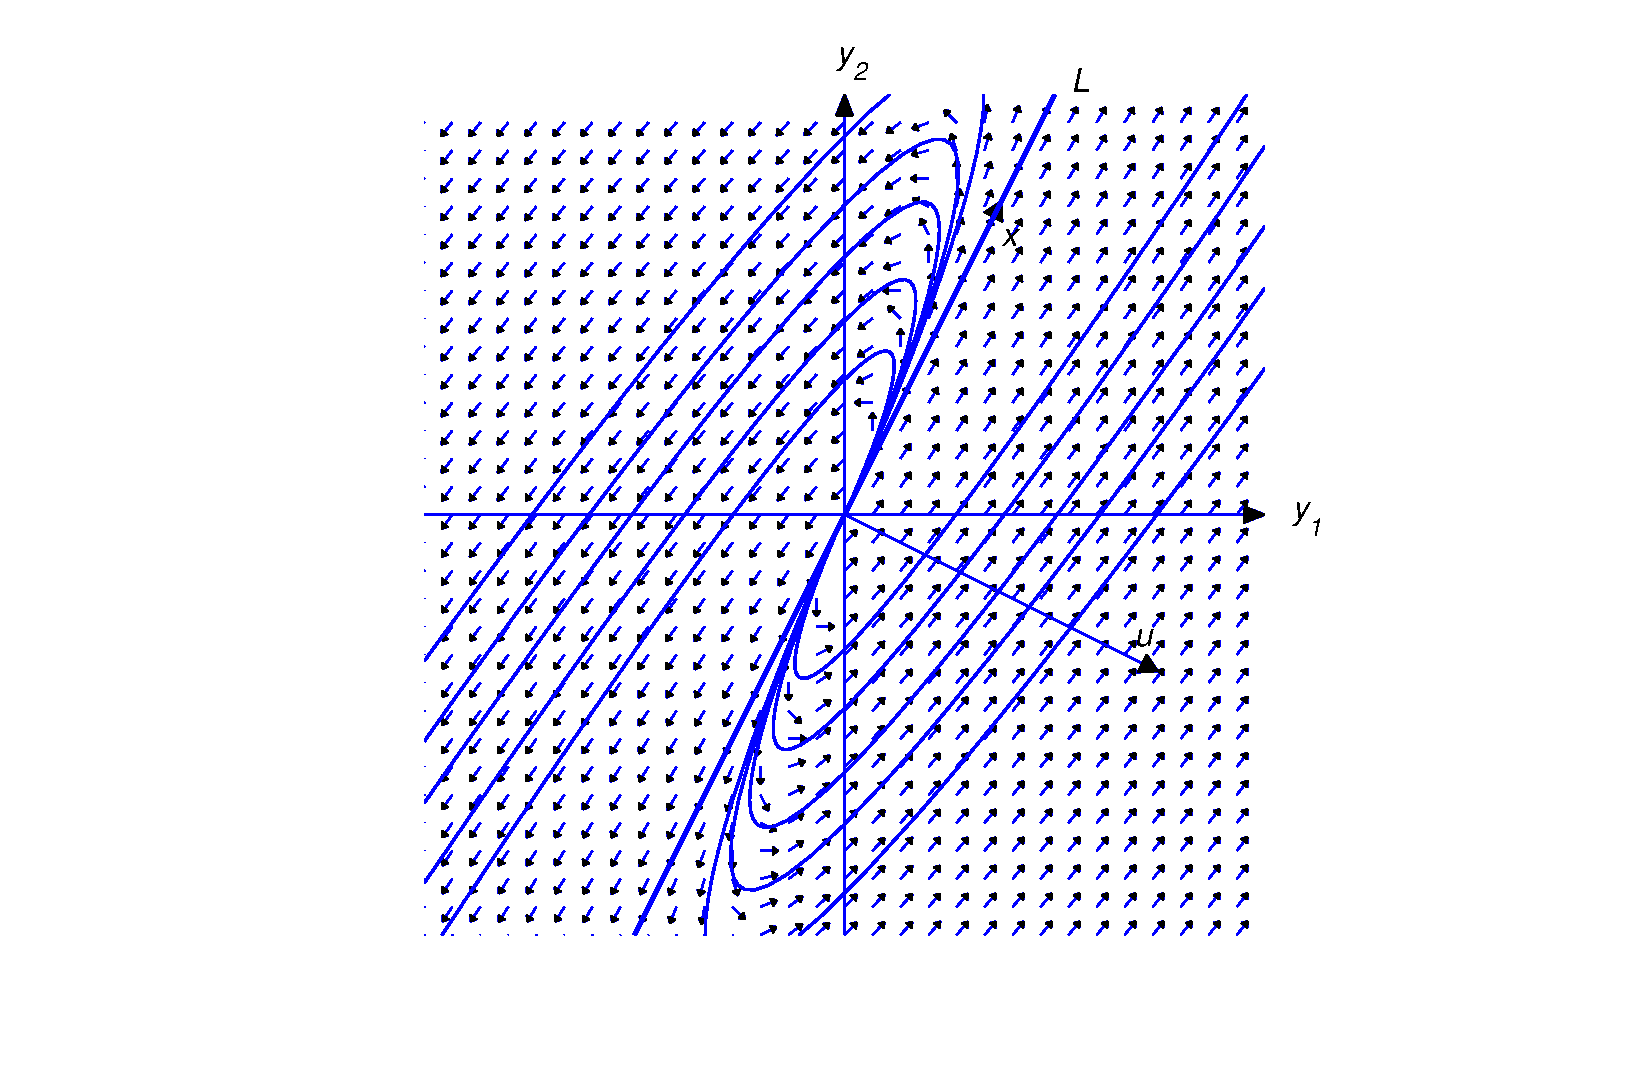
\includegraphics[bb=-78 148 689 643, width=5.67in, height=3.66in, keepaspectratio]{fig100502}}
    \caption{Positive eigenvalue; motion away from the origin}
    \label{figure:10.5.2}
  \end{minipage}
  \begin{minipage}[b]{0.5\linewidth}
    \centering
    \scalebox{.65}{
    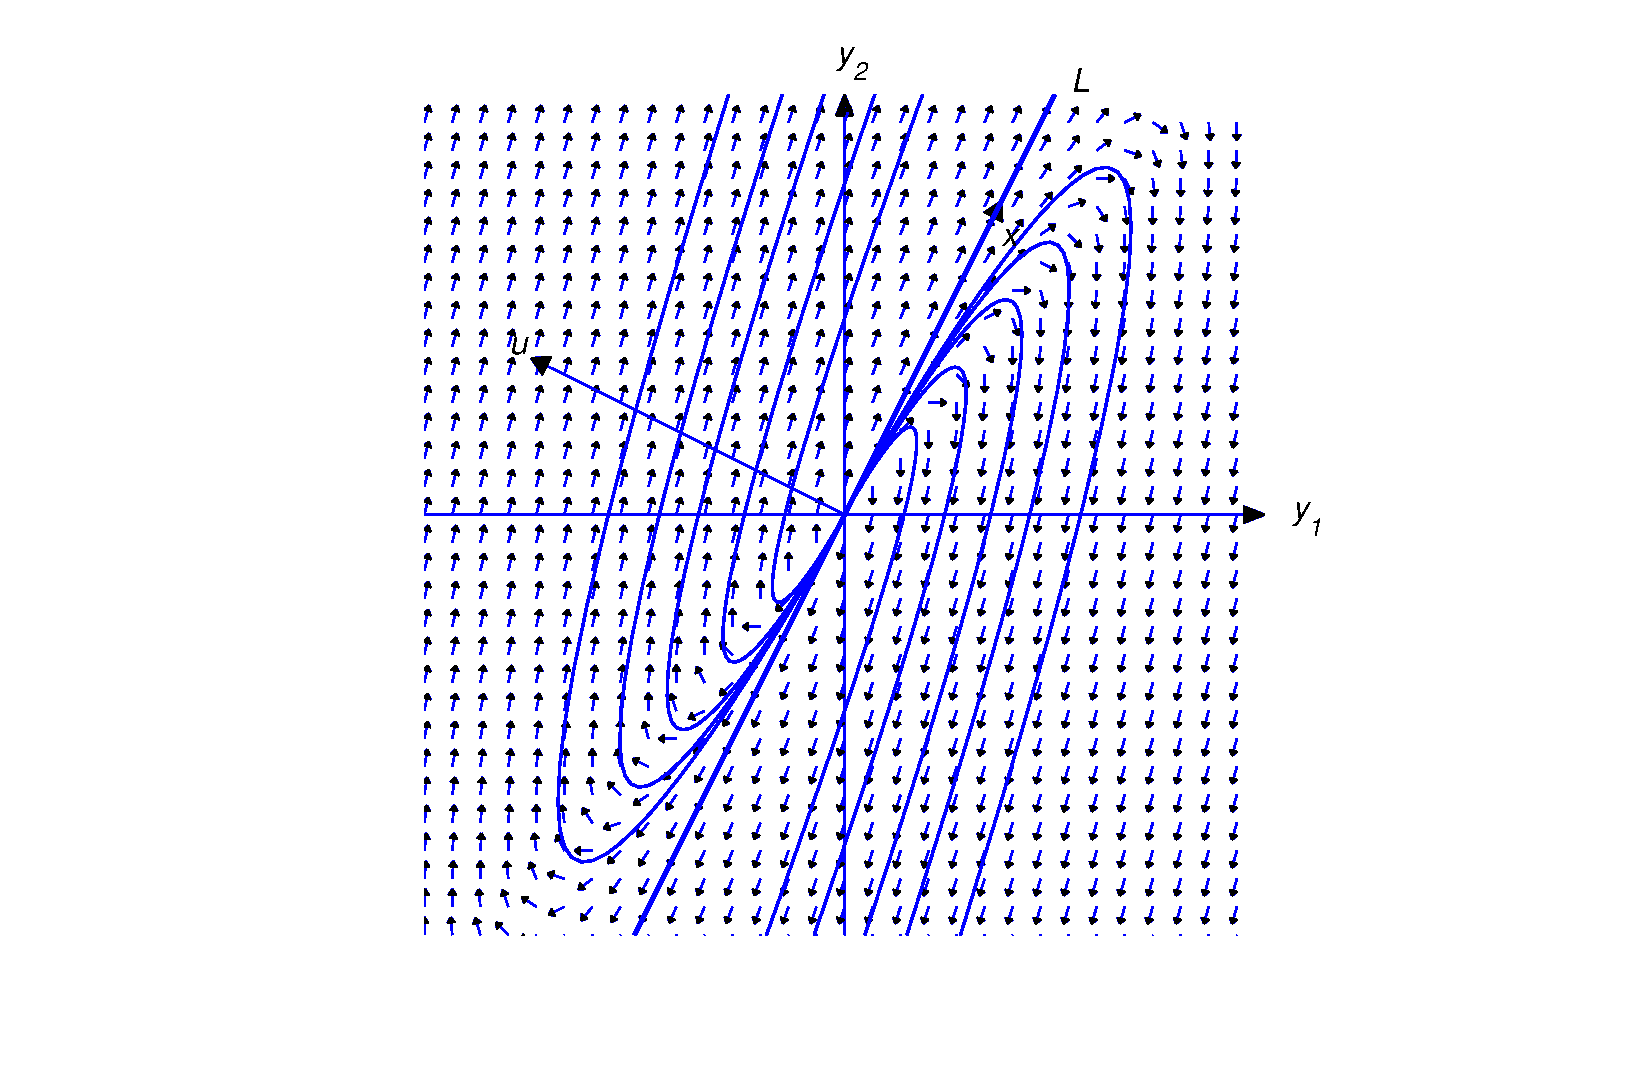
\includegraphics[bb=-78 148 689 643, width=5.67in, height=3.66in, keepaspectratio]{fig100503}}
    \caption{Positive eigenvalue; motion away from the origin}
    \label{figure:10.5.3}
  \end{minipage}
\end{figure}

\begin{figure}[H]
  \color{blue}
  \begin{minipage}[b]{0.5\linewidth}
    \centering
    \scalebox{.65}{
    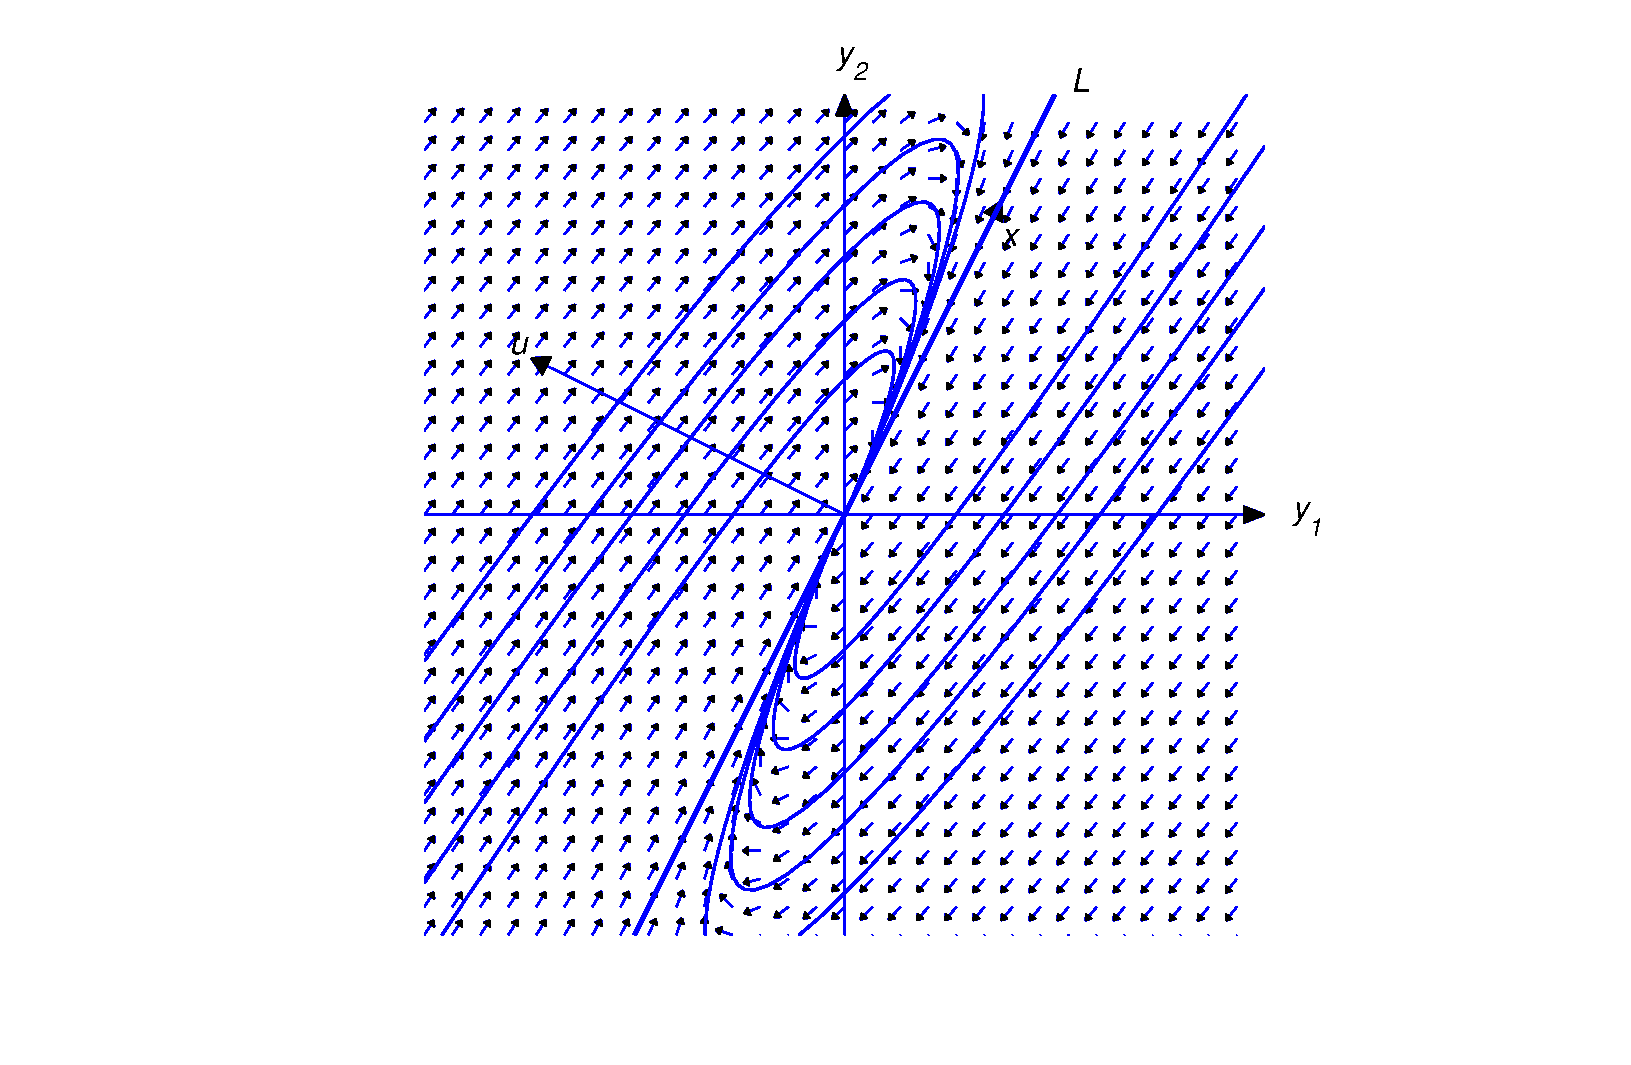
\includegraphics[bb=-78 148 689 643, width=5.67in, height=3.66in, keepaspectratio]{fig100504}
    }
    \caption{Negative eigenvalue; motion toward the origin}
    \label{figure:10.5.4}
  \end{minipage}
  \begin{minipage}[b]{0.5\linewidth}
    \centering
    \scalebox{.65}{
    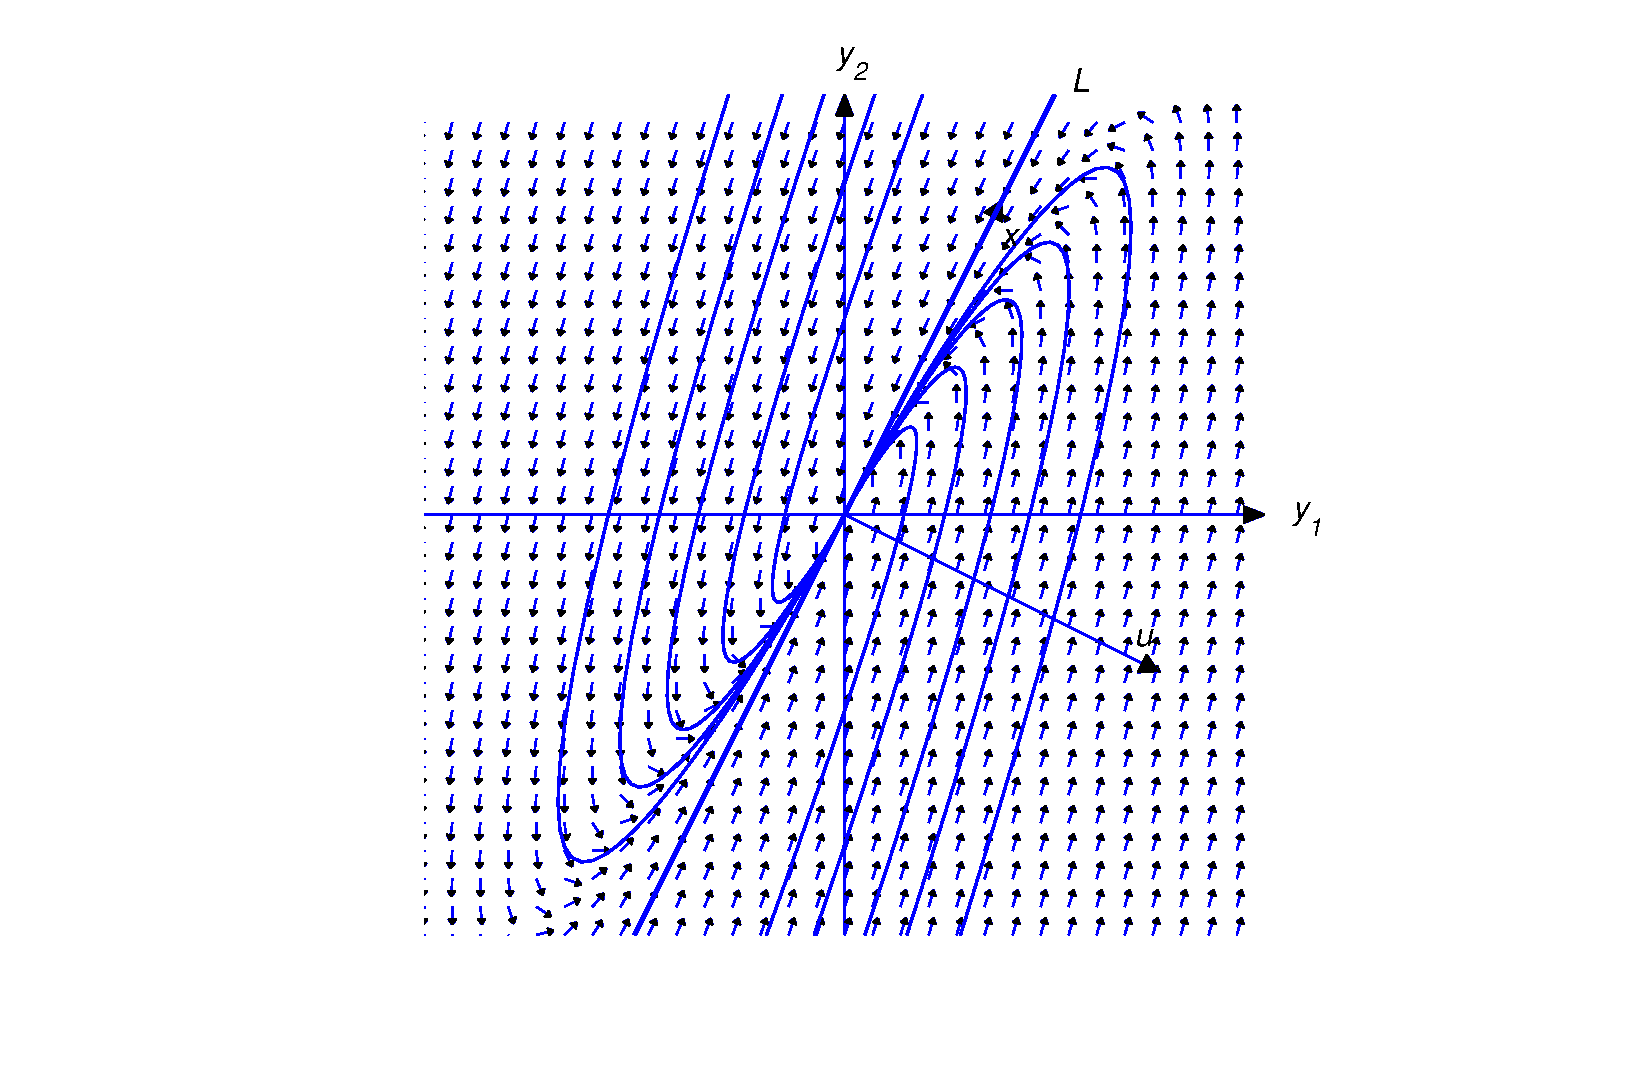
\includegraphics[bb=-78 148 689 643, width=5.67in, height=3.66in, keepaspectratio]{fig100505}
    }
    \caption{Negative eigenvalue; motion toward the origin}
    \label{figure:10.5.5}
  \end{minipage}
\end{figure}

\newpage

\exercises In Exercises~\ref{exer:10.5.1}--\ref{exer:10.5.12} find the general solution.

\begin{exerciselist}
  \begin{tabular}[t]{@{}p{168pt}@{}p{168pt}}
    \item\label{exer:10.5.1} $\dst{{\bf y}'=\twobytwo34{-1}7{\bf y}}$ &
    \item\label{exer:10.5.2} $\dst{{\bf y}'=\twobytwo0{-1}1{-2}{\bf y}}$
  \end{tabular}

  \begin{tabular}[t]{@{}p{168pt}@{}p{168pt}}
    \item\label{exer:10.5.3} $\dst{{\bf y}'=\twobytwo{-7}4{-1}{-11}{\bf y}}$ &
    \item\label{exer:10.5.4} $\dst{{\bf y}'=\twobytwo31{-1}1{\bf y}}$
  \end{tabular}

  \begin{tabular}[t]{@{}p{168pt}@{}p{168pt}}
    \item\label{exer:10.5.5} $\dst{{\bf y}'=\twobytwo4{12}{-3}{-8}{\bf y}}$ &
    \item\label{exer:10.5.6} $\dst{{\bf y'}=\twobytwo{-10}9{-4}2{\bf y}}$
  \end{tabular}

  \begin{tabular}[t]{@{}p{168pt}@{}p{168pt}}
    \item\label{exer:10.5.7} $\dst{{\bf y'}=\twobytwo{-13}{16}{-9}{11}{\bf y}}$ &
    \item\label{exer:10.5.8} $\dst{{\bf y'}=\threebythree021{-4}61042{\bf y}}$
  \end{tabular}

  \begin{tabular}[t]{@{}p{168pt}@{}p{168pt}}
    \item\label{exer:10.5.9} $\dst{{\bf y}'=\frac{1}{3}\threebythree11{-3}{-4}{-4}3{-2}10{\bf y}}$ &
    \item\label{exer:10.5.10} $\dst{{\bf y}' =\threebythree{-1}1{-1}{-2}02{-1}3{-1}{\bf y}}$
  \end{tabular}

  \begin{tabular}[t]{@{}p{168pt}@{}p{168pt}}
    \item\label{exer:10.5.11} $\dst{{\bf y}' =\threebythree4{-2}{-2}{-2}3{-1}2{-1}3{\bf y}}$ &
    \item\label{exer:10.5.12} $\dst{{\bf y}'= \threebythree6{-5}32{-1}3211{\bf y}}$
  \end{tabular}

  \exercisetext{In Exercises~\ref{exer:10.5.13}--\ref{exer:10.5.23} solve the initial value
  problem.}

  \item\label{exer:10.5.13}
        $\dst{{\bf y}'=\twobytwo{-11}8{-2}{-3}{\bf y},\quad{\bf y}(0)=\twocol62}$

  \item\label{exer:10.5.14}
        $\dst{{\bf y}'=\twobytwo{15}{-9}{16}{-9}{\bf y},\quad{\bf y}(0)=\twocol58}$

  \item\label{exer:10.5.15} $\dst{{\bf y}'=\twobytwo{-3}{-4}1{-7}{\bf y},\quad{\bf y}(0)=\twocol23}$

  \item\label{exer:10.5.16}
        $\dst{{\bf y}'=\twobytwo{-7}{24}{-6}{17}{\bf y},\quad{\bf y}(0)=\twocol31}$

  \item\label{exer:10.5.17} $\dst{{\bf y}'=\twobytwo{-7}3{-3}{-1}{\bf y},\quad{\bf y}(0)=\twocol02}$

  \item\label{exer:10.5.18}
        $\dst{{\bf y}' =\threebythree{-1}101{-1}{-2}{-1}{-1}{-1}{\bf y},\quad {\bf y}(0)=\threecol65{-7}}$

  \item\label{exer:10.5.19}
        $\dst{{\bf y}' =\threebythree{-2}21{-2}21{-3}32{\bf y},\quad {\bf y}(0)=\threecol{-6}{-2}0}$

  \item\label{exer:10.5.20}
        $\dst{{\bf y}' =\threebythree{-7}{-4}4{-1}01{-9}{-5}6{\bf y},\quad\bf {\bf y}(0)=\threecol{-6}9{-1}}$

  \item\label{exer:10.5.21}
        $\dst{{\bf y}' =\threebythree{-1}{-4}{-1}361{-3}{-2}3\bf y,\quad\bf y(0)=\threecol{-2}13}$

  \item\label{exer:10.5.22}
        $\dst{{\bf y}' =\threebythree4{-8}{-4}{-3}{-1}{-3}1{-1}9{\bf y},\quad {\bf y}(0)=\threecol{-4}1{-3}}$

  \item\label{exer:10.5.23}
        $\dst{{\bf y}'= \threebythree{-5}{-1}{11}{-7}1{13}{-4}08{\bf y},\quad {\bf y}(0)=\threecol022}$

  \exercisetext{The coefficient matrices in Exercises~\ref{exer:10.5.24}--\ref{exer:10.5.32} have
  eigenvalues of multiplicity $3$. Find the general solution.}

  \begin{tabular}[t]{@{}p{168pt}@{}p{168pt}}
    \item\label{exer:10.5.24} $\dst{{\bf y}' =\threebythree5{-1}1{-1}9{-3}{-2}24{\bf y}}$ &
    \item\label{exer:10.5.25} $\dst{{\bf y}' =\threebythree1{10}{-12}2232{-1}6{\bf y}}$
  \end{tabular}

  \begin{tabular}[t]{@{}p{168pt}@{}p{168pt}}
    \item\label{exer:10.5.26} $\dst{{\bf y}' =\threebythree{-6}{-4}{-4}2{-1}1231{\bf y}}$ &
    \item\label{exer:10.5.27} $\dst{{\bf y}' =\threebythree02{-2}{-1}5{-3}111{\bf y}}$
  \end{tabular}

  \begin{tabular}[t]{@{}p{168pt}@{}p{168pt}}
    \item\label{exer:10.5.28} $\dst{{\bf y}' =\threebythree{-2}{-12}{10}2{-24}{11}2{-24}8{\bf y}}$ &
    \item\label{exer:10.5.29} $\dst{{\bf y}' =\threebythree{-1}{-12}81{-9}41{-6}1{\bf y}}$
  \end{tabular}

  \begin{tabular}[t]{@{}p{168pt}@{}p{168pt}}
    \item\label{exer:10.5.30} $\dst{{\bf y}' =\threebythree{-4}0{-1}{-1}{-3}{-1}10{-2}{\bf y}}$ &
    \item\label{exer:10.5.31} $\dst{{\bf y}' =\threebythree{-3}{-3}445{-8}23{-5}\bf y}$
  \end{tabular}

  \item\label{exer:10.5.32} ${\bf y}'={\threebythree{-3}{-1}01{-1}0{-1}{-1}{-2}}{\bf y}$

  \item\label{exer:10.5.33} Under the assumptions of Theorem~\ref{thmtype:10.5.1}, suppose ${\bf u}$
        and $\hat{\bf u}$ are vectors such that
  \[
    (A-\lambda_{1}I){\bf u}={\bf x}\quad\mbox{and }\quad (A-\lambda_{1}I)\hat{\bf u}={\bf x},
  \]
  and let
  \[
    {\bf y}_{2}={\bf u}e^{\lambda_{1}t}+{\bf x}te^{\lambda_{1}t}\quad\mbox{and }\quad \hat{\bf y}_{2}=\hat{\bf u}e^{\lambda_{1}t}+{\bf x}te^{\lambda_{1}t}.
  \]
  Show that ${\bf y}_{2}-\hat{\bf y}_{2}$ is a scalar multiple of
  ${\bf y}_{1}={\bf x}e^{\lambda_{1}t}$.

  \item\label{exer:10.5.34} Under the assumptions of Theorem~\ref{thmtype:10.5.2}, let
  \begin{eqnarray*}
    {\bf y}_{1} & = & {\bf x}e^{\lambda_{1}t},                                      \\
    {\bf y}_{2} & = & {\bf u}e^{\lambda_{1}t}+{\bf x}te^{\lambda_{1}t},\mbox{ and } \\
    {\bf y}_{3} & = & {\bf v}e^{\lambda_{1}t}+{\bf u}te^{\lambda_{1}t}+{\bf x}{\frac{t^{2}e^{\lambda_{1}t}}{2}}.
  \end{eqnarray*}
  Complete the proof of Theorem~\ref{thmtype:10.5.2} by showing that ${\bf y}_{3}$ is a solution of
  ${\bf y}'=A{\bf y}$ and that $\{{\bf y}_{1},{\bf y}_{2},{\bf y}_{3}\}$ is linearly independent.

  \item\label{exer:10.5.35} Suppose the matrix
  \[
    A=\left[
    \begin{array}{cc}
      a_{11} & a_{12} \\
      a_{21} & a_{22}
    \end{array}\right]
  \]
  has a repeated eigenvalue $\lambda_{1}$ and the associated eigenspace is one-dimensional. Let
  ${\bf x}$ be a $\lambda_{1}$-eigenvector of $A$. Show that if
  $(A-\lambda_{1}I){\bf u}_{1}={\bf x}$ and $(A-\lambda_{1}I){\bf u}_{2}={\bf x}$, then
  ${\bf u}_{2}-{\bf u}_{1}$ is parallel to ${\bf x}$. Conclude from this that all vectors ${\bf u}$
  such that $(A-\lambda_{1}I){\bf u}={\bf x}$ define the same positive and negative half-planes with
  respect to the line $L$ through the origin parallel to ${\bf x}$.

  \exercisetext{In Exercises~\ref{exer:10.5.36}-~\ref{exer:10.5.45} plot trajectories of the given
  system.}
  \begin{tabular}[t]{@{}p{168pt}@{}p{168pt}}
    \item\label{exer:10.5.36} \CGex\, ${\bf y}'=\dst{\twobytwo{-3}{-1}41}{\bf y}$ &
    \item\label{exer:10.5.37} \CGex\, ${\bf y}'=\dst{\twobytwo2{-1}10}{\bf y}$
  \end{tabular}

  \begin{tabular}[t]{@{}p{168pt}@{}p{168pt}}
    \item\label{exer:10.5.38} \CGex\, ${\bf y}'=\dst{\twobytwo{-1}{-3}35}{\bf y}$ &
    \item\label{exer:10.5.39} \CGex\, ${\bf y}'=\dst{\twobytwo{-5}3{-3}1}{\bf y}$
  \end{tabular}

  \begin{tabular}[t]{@{}p{168pt}@{}p{168pt}}
    \item\label{exer:10.5.40} \CGex\, ${\bf y}'=\dst{\twobytwo{-2}{-3}34}{\bf y}$ &
    \item\label{exer:10.5.41} \CGex\, ${\bf y}'=\dst{\twobytwo{-4}{-3}32}{\bf y}$
  \end{tabular}

  \begin{tabular}[t]{@{}p{168pt}@{}p{168pt}}
    \item\label{exer:10.5.42} \CGex\, ${\bf y}'=\dst{\twobytwo0{-1}1{-2}}{\bf y}$ &
    \item\label{exer:10.5.43} \CGex\, ${\bf y}'=\dst{\twobytwo01{-1}2}{\bf y}$
  \end{tabular}

  \begin{tabular}[t]{@{}p{168pt}@{}p{168pt}}
    \item\label{exer:10.5.44} \CGex\, ${\bf y}'=\dst{\twobytwo{-2}1{-1}0}{\bf y}$ &
    \item\label{exer:10.5.45} \CGex\, ${\bf y}'=\dst{\twobytwo0{-4}1{-4}}{\bf y}$
  \end{tabular}
\end{exerciselist}
